% !TEX root = main.tex

\section{传输层} % transport layer
传输层协议称为\textbf{端到端}或\textbf{进程到进程}的协议。 因特网的传输层可以为两个进程在\textbf{不可靠的网络层}上建立一条\textbf{可靠的逻辑链路},可以提供\textbf{字节流}传输服务,并且可以进行\textbf{流控制}和\textbf{拥塞控制}。

因特网的传输层有两个协议: UDP和TCP。
UDP协议提供不可靠的尽力服务, TCP协议提供可靠的字节流服务。
协议号:TCP为6,ICMP=1;UDP为17,IGMP=2

TCP/UDP通过数据段(segment)中的目的端口号(2B)确定将收到的数据段交给上层哪个进程。
\begin{itemize}
    \item 知名端口:0-1023,为提供知名网络服务的系统进程所用。    例如: 80-HTTP, 21-ftp Control, 20-ftp Data, 23-telnet,25-SMTP, 110-POP3,53-DNS
    \item 注册端口:1024-49151。在IANA注册的专用端口号,为企业软件所用。
    \item 动态端口:49152-65535,没有规定用途的端口号,一般用户可以随意使用。也称为私    用或暂用端口号。
\end{itemize}

\subsection{UDP协议}
用户数据报协议(User Datagram Protocol, UDP)只提供\textbf{无连接的不可靠的尽力服务}。发送给接收进程的数据有可能丢失,也有可能错序。
可以说UDP协议是IP协议的简单扩展,在IP协议上增加了\textbf{端口号},把进程关联起来了。

接收进程每次接收一个完整的数据报,如果进程设置的接收缓冲区不够大,收到的数据报将被截断。

数据报的内容
\begin{itemize}
    \item 总长度:整个UDP报文长度
    \item 源端口号和目的端口号:用于关联发送进程和接收进程
    \item 校验和:由\textbf{伪IP头(就是用来算校验和用)}、 UDP头(校验和为0)和UDP数据形成。其中,伪IP头的协议号为17。如果发送方把校验和设置为0,接收方会忽略校验和。 UDP长度就是UDP头部的总长度。
\end{itemize}


\subsection{TCP协议}
传输控制协议(Transmission Control Protocol, TCP)为进程之间提供\textbf{面向连接的可靠的}数据传送服务(通过滑动窗口协议实现)。TCP为\textbf{全双工}协议。TCP提供\textbf{流控制}机制,即控制发送方的发送速度,使发送的数据不会淹没接收方。作为因特网的主要数据发源地,TCP还提供\textbf{拥塞控制}功能。
\begin{figure}[H]
    \centering
    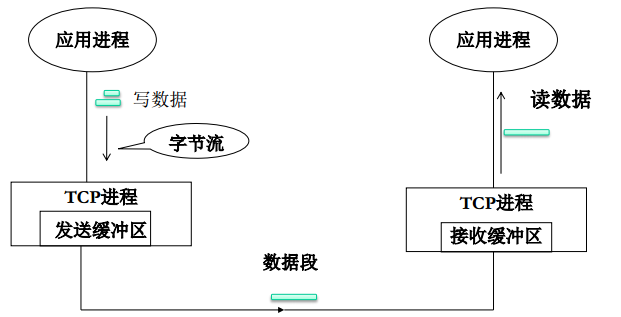
\includegraphics[width=0.5\linewidth]{fig/TCP.PNG}
\end{figure}

\begin{itemize}
\item 一个TCP连接提供\textbf{可靠的字节流服务}。字节流服务表示\textbf{没有消息边界}。例如,多次发送的数据可以放在一个数据段中传送且\textbf{不标识边界}。
\item 每个数据段的数据部分的最大长度(字节)不能超过MSS(Maximum Segment Size)。
\item 每个TCP连接可以由四元组唯一标识:\underline{源IP地址、源端口号、目的IP地址、目的端口号},通过\textbf{端口号}区分不同进程。
\item 客户端通过查路由表知道\textbf{IP地址},\textbf{端口号}自动选一个未用的
\end{itemize}

TCP数据报格式:头部长度以四个字节为单位。校验和由伪IP头、 TCP头和TCP数据部分形成。其形成方法与UDP协议类似。
\begin{itemize}
\item SYN:表示建立连接
\item FIN:表示关闭连接,不再发送数据,但是可以接收数据,也可以发送\textbf{数据段}(不包含数据)
\item ACK:表示响应
\item PSH:将接收缓冲区的进程全部推给接收方进程
\item RST:发现连接可能出了问题,连接重置
\item URG:紧急指针用于指出紧急/带外数据(out-of-band)的边界,紧急数据最后一个字节
\end{itemize}

TCP协议工作过程
\begin{center}
    \begin{tikzcd}
        \text{建立连接}\arrow{r} & \text{传送数据} & \text{释放连接}
    \end{tikzcd}
\end{center}
\begin{itemize}
    \item 建立连接:非对称活动,服务器一直在等,客户向服务器呼叫
    \item 传送数据:全双工方式
    \item 释放连接:对称活动,可由任何一方发起
\end{itemize}

三次握手建立连接:x,y为初始序号,随机数
\begin{itemize}
    \item SYN,Seq\#=x
    \item (Client)SYN+ACK,Seq\#=y; Ack\#=x+1
    \item ACK,Ack\#=y+1
\end{itemize}
这里确认号含义与数据链路层不同,这里是\textcolor{red}{\textbf{期待接收}}的序号

四次握手关闭连接
\begin{itemize}
    \item FIN,Seq\#=x
    \item (Client)ACK,Ack\#=x+1
    \item (Client)FIN,Seq\#=y
    \item ACK,Ack\#=y+1
\end{itemize}
可以合并中间两次握手(ACK和FIN)或两方同时发出ACK

先发送FIN报文的一方在ACK发送完毕后需要等待2MSL(Maximum Segment Lifetime)的时间才\textbf{完全关闭}连接(占用端口号)。 TCP标准中MSL采用60秒, Unix采用30秒。
\begin{figure}[H]
    \centering
    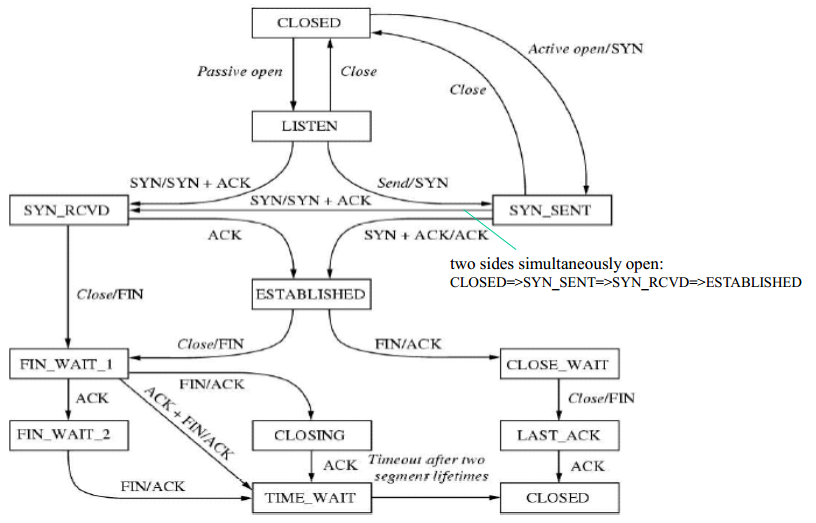
\includegraphics[width=0.8\linewidth]{fig/TCP-transition.PNG}
\end{figure}

TCP协议使用\textbf{选择性确认}协议,不使用NAK。只有\textbf{一个超时定时器}。
\begin{itemize}
\item 采用字节流方式,每个数据段使用其第一个字节的编号作为序号,按字节编号。
\item 确认号为期待接收的下一个字节(下一个数据段)的序号。
\item 由于TCP是对IP数据报的封装,要获取数据的长度,可以通过IP数据报中的总长度获取。
\item TCP协议没有说明如何处理错序到达的数据段,要取决于具体实现。
\end{itemize}

\begin{figure}[H]
    \centering
    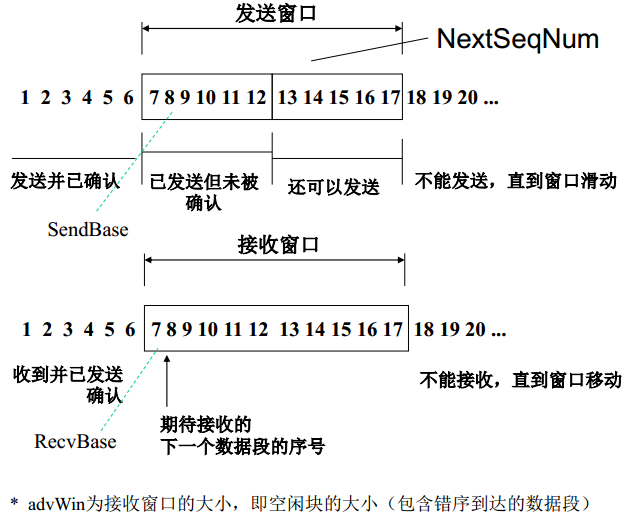
\includegraphics[width=0.8\linewidth]{fig/TCP-window.PNG}
\end{figure}

\begin{itemize}
\item 接收方先传MSS,x和接收窗口大小(advWin)
\item 发送方做发送窗口,序号为x+1,大小等同advWin大小
\item 接收窗口大小\textbf{会变},不同于数据链路层;同理发送窗口大小\textbf{也会改变},用接收窗口大小设置发送窗口大小
\item 要等接收方进程将缓冲区取空,发送方才能继续发,否则发送窗口大小始终为0
\item 会自动移动超时定时器
\item 一旦发现有问题,立即减慢
\item 要考虑错序到达的数据段
\end{itemize}